%%%%%%%%%%%%%%%%%%%%%%%%%%%%%%%%%%%%%%
% LaTeX poster template
% Created by Nathaniel Johnston
% August 2009
% http://www.nathanieljohnston.com/2009/08/latex-poster-template/
%%%%%%%%%%%%%%%%%%%%%%%%%%%%%%%%%%%%%%

\documentclass[final]{beamer}
\usepackage[scale=1.24]{beamerposter}
\usepackage{graphicx}
\usepackage{adjustbox}
\usepackage{subcaption}
\usepackage{array}
\usepackage{booktabs}
%-----------------------------------------------------------
% Define the column width and poster size
% To set effective sepwid, onecolwid and twocolwid values, first choose how many columns you want and how much separation you want between columns
% The separation I chose is 0.024 and I want 4 columns
% Then set onecolwid to be (1-(4+1)*0.024)/4 = 0.22
% Set twocolwid to be 2*onecolwid + sepwid = 0.464
%-----------------------------------------------------------

\newlength{\sepwid}
\setlength{\paperwidth}{48in}
\setlength{\paperheight}{27in}
\setlength{\sepwid}{0.024\paperwidth}

%% Four columns
%% \newlength{\onecolwid}
%% \newlength{\twocolwid}
%% \newlength{\threecolwid}
%% \setlength{\onecolwid}{0.22\paperwidth}
%% \setlength{\twocolwid}{0.464\paperwidth}
%% \setlength{\threecolwid}{0.708\paperwidth}

%% Five columns
\setlength{\sepwid}{0.024\paperwidth}
\newlength{\onecolwid}
\setlength{\onecolwid}{0.171\paperwidth}
\newlength{\twocolwid}
\setlength{\twocolwid}{0.366\paperwidth}
\newlength{\threecolwid}
\setlength{\threecolwid}{0.562\paperwidth}
\newlength{\fourcolwid}
\setlength{\fourcolwid}{0.757\paperwidth}
\newlength{\fivecolwid}
\setlength{\fivecolwid}{0.952\paperwidth}

\setlength{\topmargin}{-0.5in}
\usetheme{confposter}
\usepackage{exscale}

%-----------------------------------------------------------
% The next part fixes a problem with figure numbering. Thanks Nishan!
% When including a figure in your poster, be sure that the commands are typed in the following order:
% \begin{figure}
% \includegraphics[...]{...}
% \caption{...}
% \end{figure}
% That is, put the \caption after the \includegraphics
%-----------------------------------------------------------

\usecaptiontemplate{
\small
\structure{\insertcaptionname~\insertcaptionnumber:}
\insertcaption}

%-----------------------------------------------------------
% Define colours (see beamerthemeconfposter.sty to change these colour definitions)
%-----------------------------------------------------------

%\setbeamercolor{block title}{fg=iclrgreen,bg=white}
%\setbeamercolor{block body}{fg=black,bg=white}
%\setbeamercolor{block alerted title}{fg=white,bg=dblue!70}
%\setbeamercolor{block alerted body}{fg=black,bg=dblue!10}





\usepackage{tikz}
\usetikzlibrary{shapes.geometric, arrows, shapes.symbols, shadows, patterns}

\tikzstyle{start} = [rectangle, draw, text centered, rounded corners, align=center, minimum height=2em]
\tikzstyle{process} = [rectangle, draw, text centered, minimum height=2em]
\tikzstyle{data}=[trapezium, draw, text centered, trapezium left angle=60, trapezium right angle=120, minimum height=2em]
\tikzstyle{connector} = [draw, -latex']
\tikzstyle{cloud} = [cloud, draw, text centered, cloud puffs=10, cloud ignores aspect, minimum height=2em]
\tikzset{
  multidocument/.style={
    shape=tape,
    draw,
    fill=white,
    outer sep=3pt,
    tape bend top=none,
    double copy shadow},
  singledocument/.style={
    shape=tape,
    draw,
    fill=white,
    tape bend top=none},
  database/.style={
    cylinder,
    shape border rotate=90,
    aspect=0.1,
    align=center,
    draw}
}
\usetikzlibrary{positioning}

\usepackage{float}



%-----------------------------------------------------------
% Name and authors of poster/paper/research
%-----------------------------------------------------------

\title[ForecastBench]{ForecastBench: A Dynamic Benchmark of AI Forecasting Capabilities}
\author[ForecastBench Team]{Ezra Karger\inst{1,2} \and Houtan Bastani\inst{1} \and Chen Yueh-Han\inst{3} \and Zachary Jacobs\inst{1} \and Danny Halawi\inst{4} \and Fred Zhang\inst{4} \and Philip E. Tetlock\inst{1,5}}
\institute[]{
  \inst{1} Forecasting Research Institute
  \inst{2} Federal Reserve Bank of Chicago
  \inst{3} New York University
  \inst{4} University of California, Berkeley
  \inst{5} University of Pennsylvania
}
\date[ICLR 2025]{ICLR 2025: April 24-28}

%-----------------------------------------------------------
% Start the poster itself
%-----------------------------------------------------------

\begin{document}
\begin{frame}[t]
  \begin{columns}[t]

    \begin{column}{\sepwid}\end{column}

    \begin{column}{\onecolwid}

      \setbeamercolor{block alerted title}{fg=black,bg=iclrblue}
      \setbeamercolor{block alerted body}{fg=black,bg=white}
      \begin{alertblock}{Motivation}
        Like math and coding, forecasting is a useful testbed of LLM reasoning ability.
        \vskip2ex
        Forecasting is a real-world task that guides the decisions of individuals and organizations on a daily basis.
      \end{alertblock}

      \vskip2ex

      \begin{block}{Benchmark Features}
        \begin{itemize}
        \item Continuously updated with questions about future events\\
          $\Rightarrow$ \textbf{immune to look-ahead bias}
        \item Periodic surveys of the general public and superforecasters\\
          $\Rightarrow$ \textbf{human comparison}
        \item Fully automated with open source codebase\\
          $\Rightarrow$ \textbf{verifiable}
        \item Publicly available leaderboards\\
          $\Rightarrow$ \textbf{updated nightly}
        \item Datasets released regularly to GitHub and Hugging Face\\
          $\Rightarrow$ \textbf{train your models}
        \item Maintained until at least mid-2027, thanks to a grant from \href{https://www.openphilanthropy.org/}{Open Philanthropy}!\\
          $\Rightarrow$ \textbf{stable}
        \end{itemize}
      \end{block}

      \vskip2ex

      \begin{block}{Models Tested}
        GPT-3.5-Turbo-Instruct, GPT-4, GPT-4o, Llama-2-70B, Llama-3-7B, Llama-3-
70B, Mistral-7B, Mixtral-8x7B, Mixtral-8x22B, Mistral-Large,
Qwen1.5-110B-Chat, Claude-2.1, Claude-3-Haiku, Claude-3.5-
Sonnet, Claude-3-Opus, Gemini 1.5 Flash, and Gemini 1.5 Pro.
      \end{block}


      \vskip2ex

      \setbeamercolor{block alerted title}{fg=black,bg=iclryellow}
      \setbeamercolor{block alerted body}{fg=black,bg=white}
      \begin{alertblock}{Participate}
        Benchmark your model's forecasting abilities in one of our bi-weekly forecasting rounds.\\
        \vskip2ex
        To participate, email us:\\ \texttt{forecastbench@forecastingresearch.org}
      \end{alertblock}

    \end{column}



    \begin{column}{\sepwid}\end{column}




    \begin{column}{\twocolwid}
      \begin{block}{LLMs not yet at superforecaster level}
        \begin{table}[ht!]
\centering
\tiny
\resizebox{0.75\columnwidth}{!}{%
\begin{tabular}{@{}l l l >{\centering\arraybackslash}m{2cm} >{\centering\arraybackslash}m{2cm} >{\centering\arraybackslash}m{2cm}@{}}
\toprule
Model & \begin{tabular}[c]{@{}l@{}}Information\\ provided\end{tabular} & Prompt & \begin{tabular}[c]{@{}l@{}}Dataset\\($N$=422)\end{tabular} & \begin{tabular}[c]{@{}l@{}}Market\\($N$=76)\end{tabular} & \begin{tabular}[c]{@{}l@{}}Overall\\($N$=498)\end{tabular} \\
\midrule
Superforecaster median forecast & -- & -- & 0.118 & 0.074 & 0.096 \\
Public median forecast           & -- & -- & 0.153 & 0.089 & 0.121 \\
Claude-3-5-Sonnet-20240620       & Freeze values & Scratchpad & 0.138 & 0.107 & 0.122 \\
Claude-3-5-Sonnet-20240620       & News with freeze values & Scratchpad & 0.142 & 0.112 & 0.127 \\
GPT-4-Turbo-2024-04-09          & Freeze values & Zero shot  & 0.162 & 0.095 & 0.128 \\
Claude-3-5-Sonnet-20240620       & Freeze values & Zero shot  & 0.145 & 0.117 & 0.131 \\
GPT-4                          & Freeze values & Zero shot  & 0.167 & 0.096 & 0.132 \\
GPT-4o                         & News with freeze values & Scratchpad & 0.162 & 0.105 & 0.133 \\
Claude-3-5-Sonnet-20240620       & -- & Scratchpad & 0.138 & 0.133 & 0.136 \\
GPT-4o                         & Freeze values & Scratchpad & 0.161 & 0.113 & 0.137 \\
\bottomrule
\end{tabular}
}
\end{table}

      \end{block}

      \vskip2ex

      \begin{block}{When could AI achieve superforecaster-level capabilities?}
        \begin{figure}[htb]
    \centering
    \begin{minipage}{\textwidth}
    \begin{subfigure}[t]{0.475\textwidth}
        \centering
        \begin{tikzpicture}
            \node[anchor=south west,inner sep=0] (image) at (0,0) {
                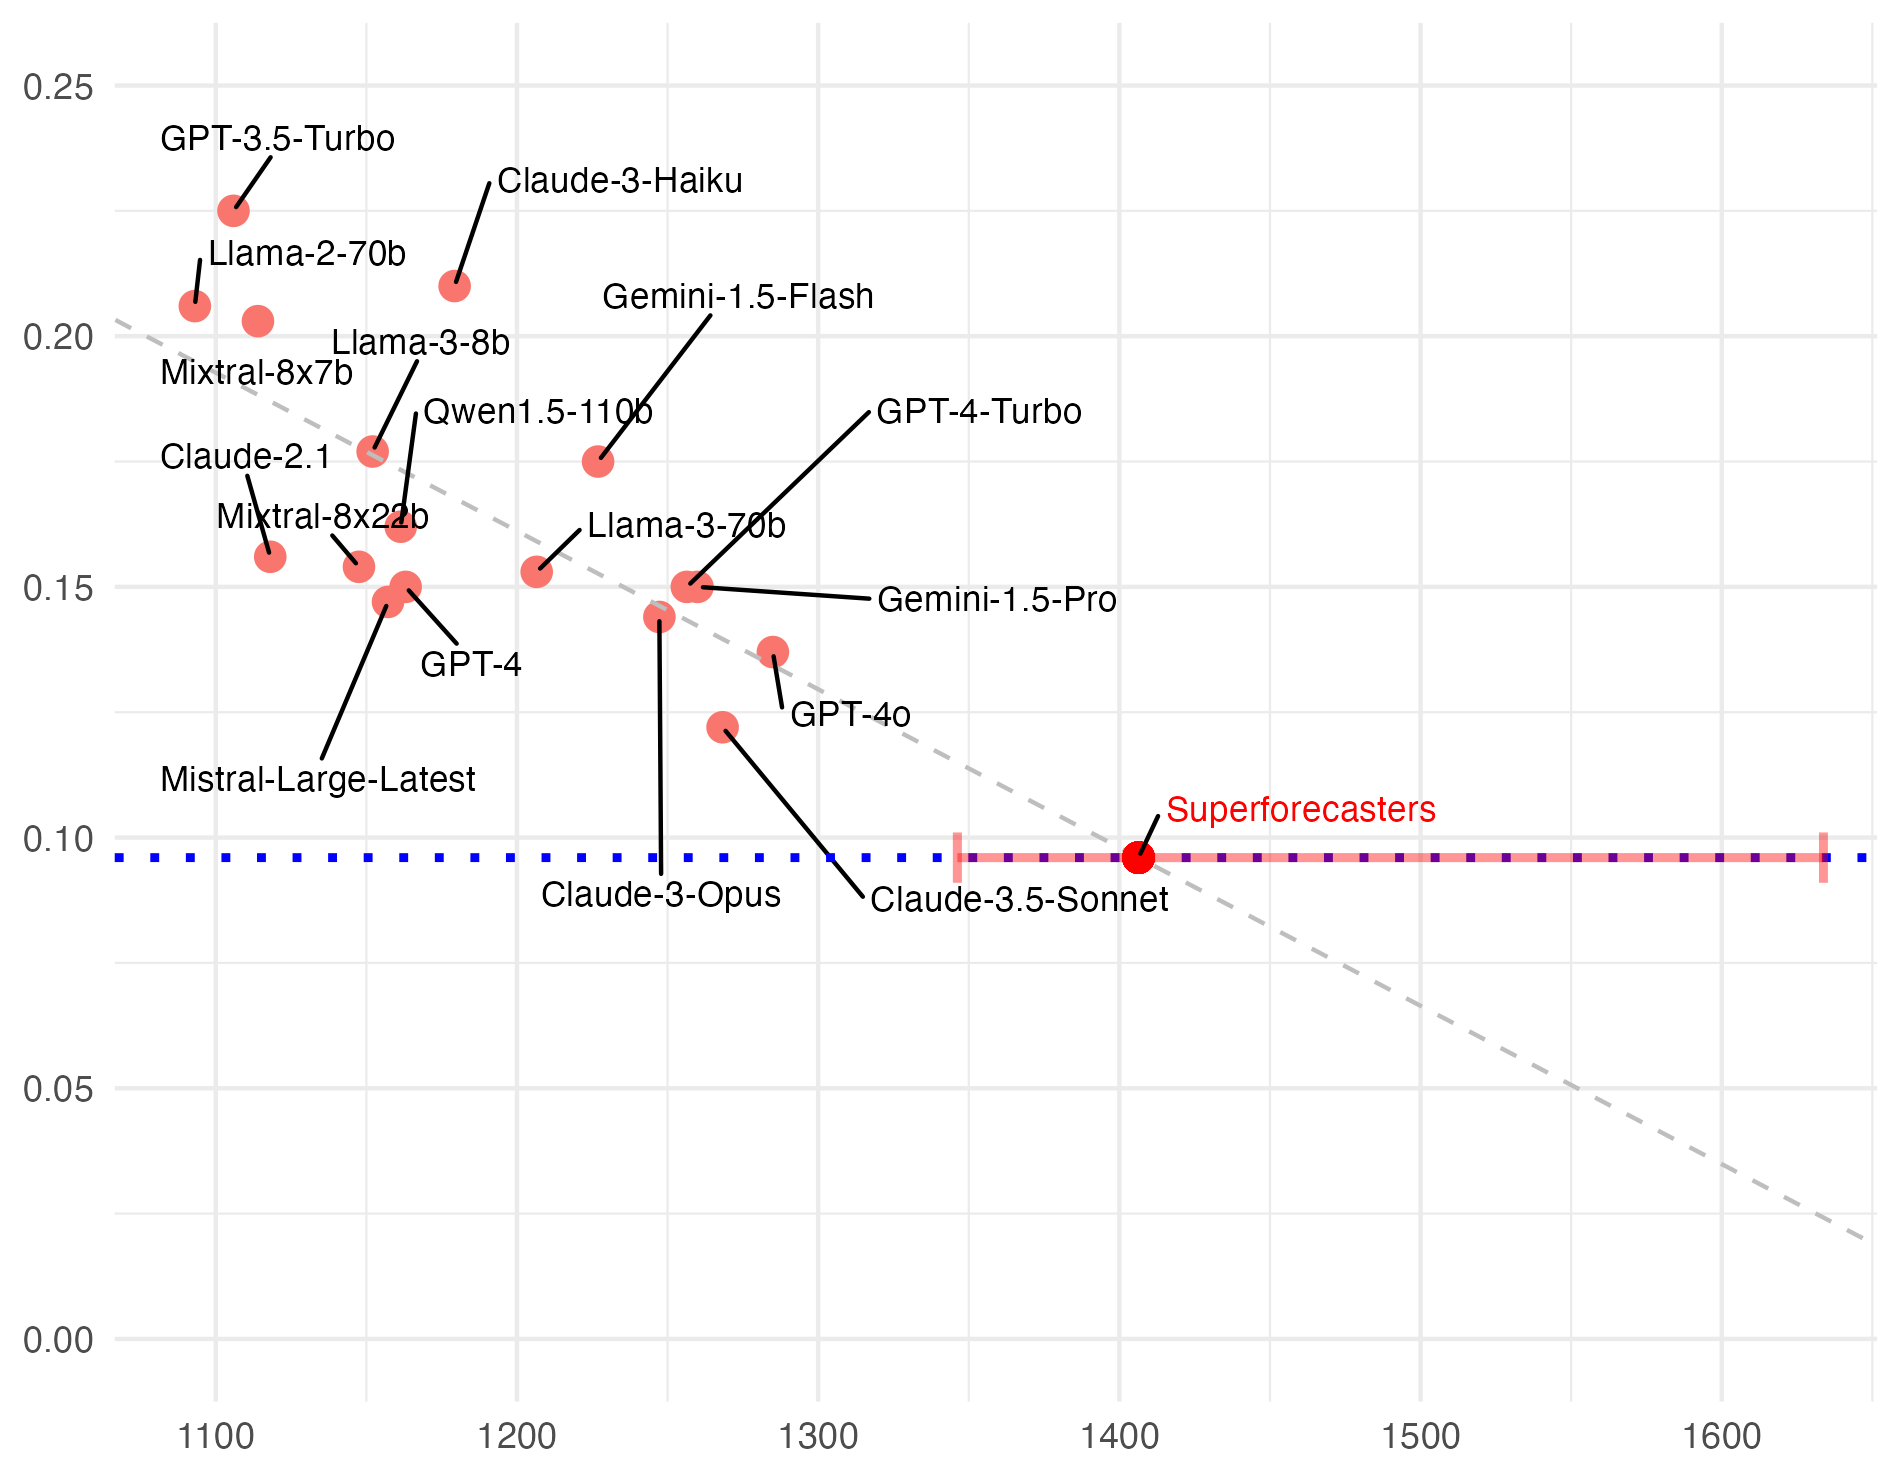
\includegraphics[width=\textwidth]{../arena_v_overall.png}
            };
            \begin{scope}[x={(image.south east)},y={(image.north west)}]
                % Add x-axis label
                \node[below,scale=0.8] at (0.5,0) {Chatbot Arena score (higher is better)};
                \node[rotate=90,left,scale=0.8] at (-0.02,.85) {Brier score (lower is better)};
            \end{scope}
        \end{tikzpicture}
    \end{subfigure}%
    \hspace*{1em}%
    \begin{subfigure}[t]{0.475\textwidth}
        \centering
        \begin{tikzpicture}
            \node[anchor=south west,inner sep=0] (image) at (0,0) {
                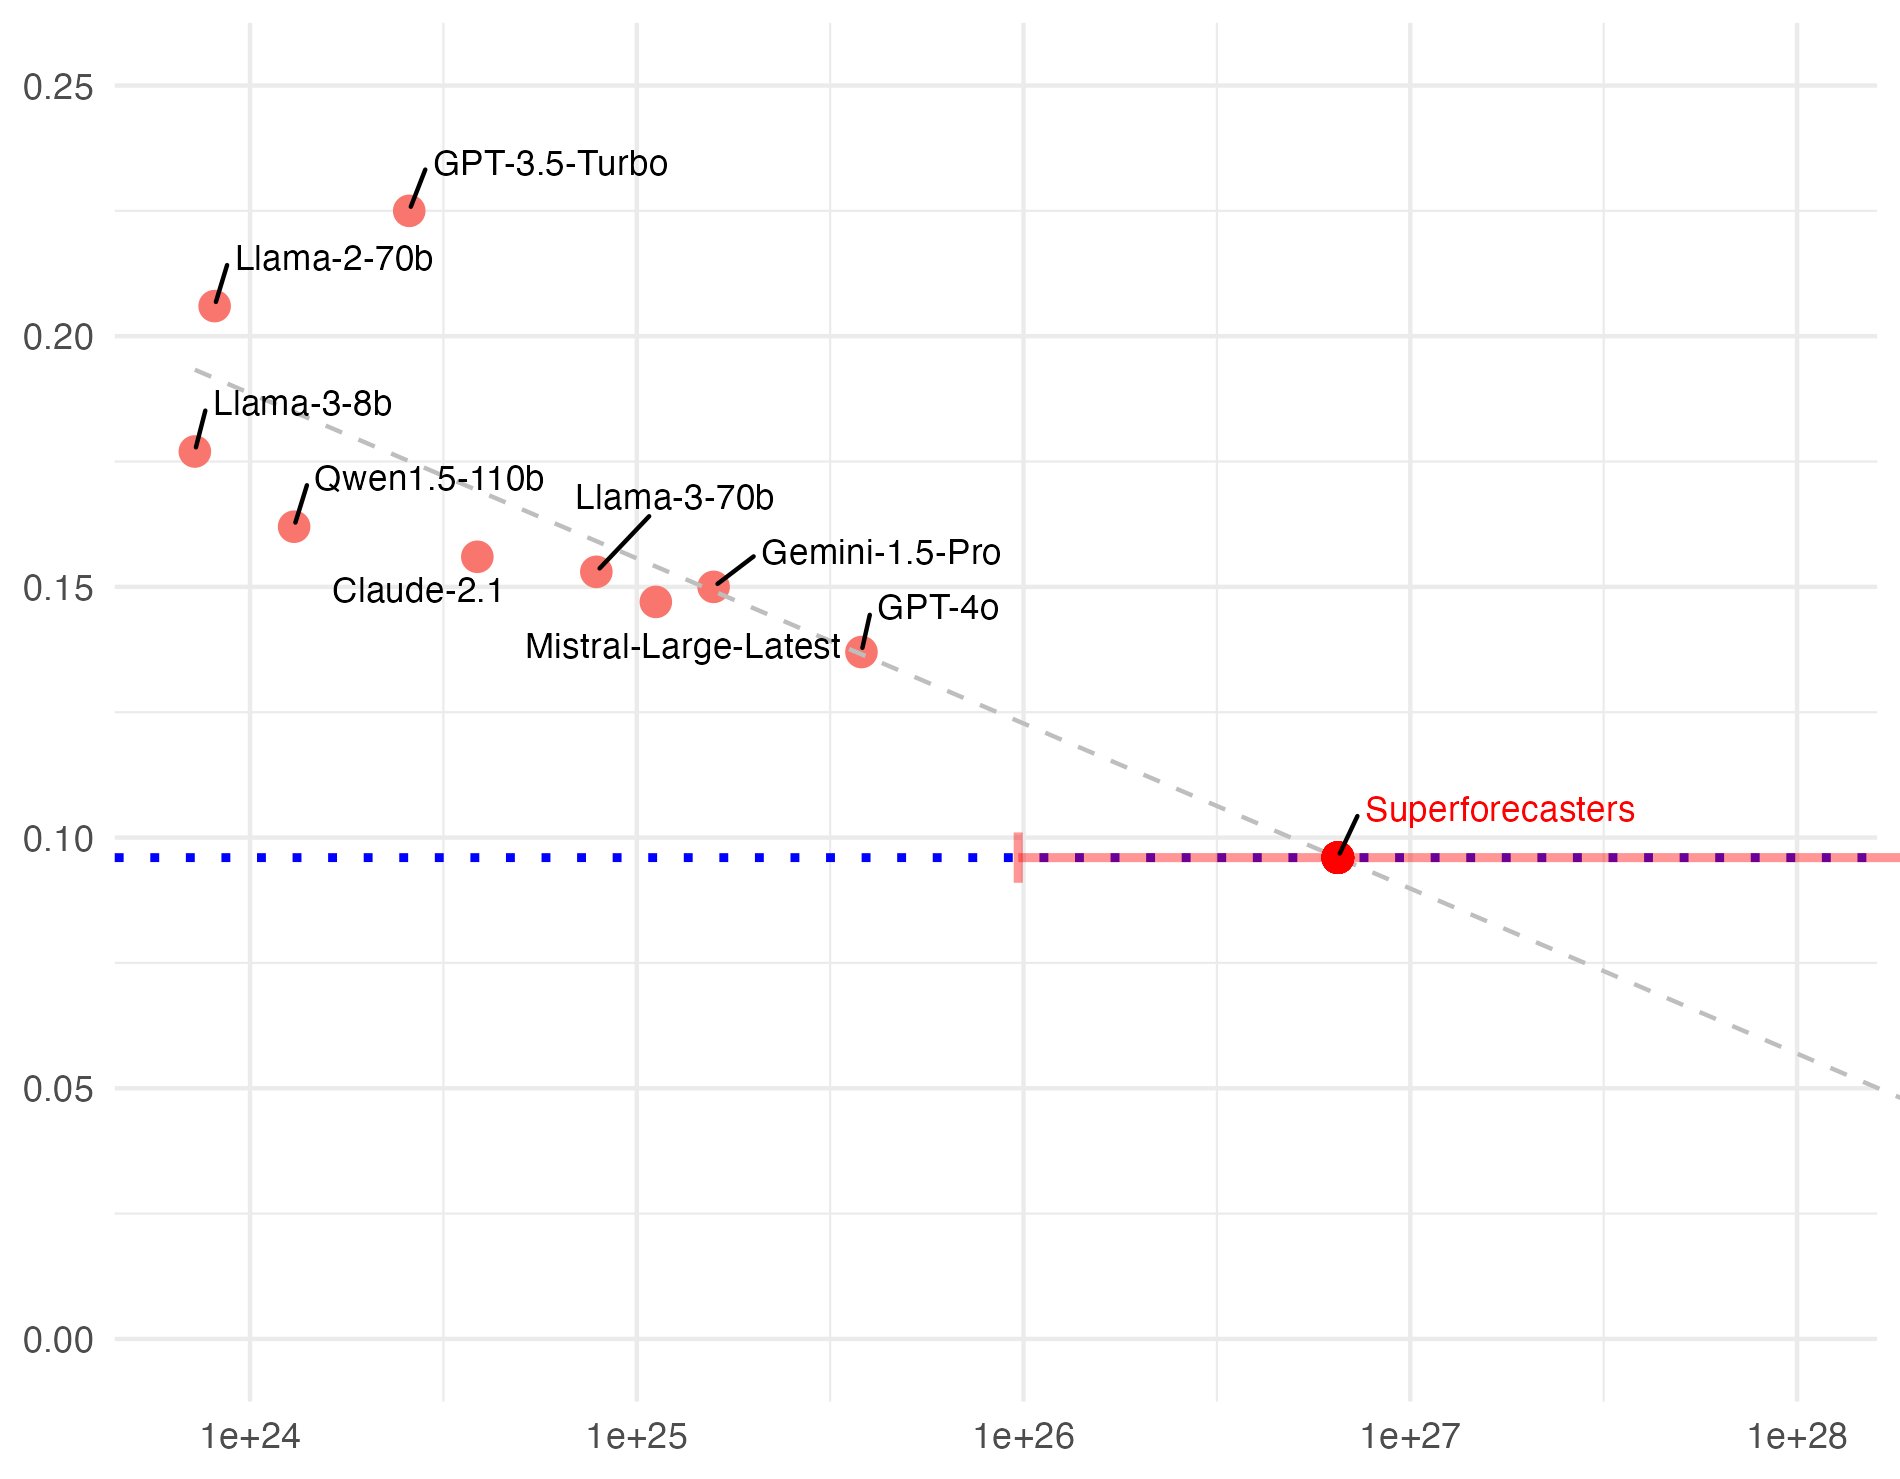
\includegraphics[width=\textwidth]{../tc_v_overall.png}
            };
            \begin{scope}[x={(image.south east)},y={(image.north west)}]
                % Add x-axis label
                \node[below,scale=0.8] at (0.5,0) {Log training compute (FLOP)};
                \node[rotate=90,left,scale=0.8] at (-0.02,.85) {Brier score (lower is better)};
            \end{scope}
        \end{tikzpicture}
    \end{subfigure}
    \end{minipage}
\end{figure}

      \end{block}

      \vskip2ex

      \setbeamercolor{block alerted title}{fg=black,bg=iclrblue}
      \setbeamercolor{block alerted body}{fg=black,bg=white}
      \begin{alertblock}{Find Us}
        Website: \href{https://www.forecastbench.org/}{\texttt{https://www.forecastbench.org}}
        \vskip2ex
        Code (MIT License):
        \raisebox{-0.15em}{
\includegraphics[height=1em]{github.png}}\hspace{0.5em}\href{https://github.com/forecastingresearch/forecastbench}{\texttt{https://github.com/forecastingresearch/forecastbench}}
        \vskip2ex
        Datasets (CC-BY-SA-4.0 License):\\
        \raisebox{-0.15em}{
\includegraphics[height=1em]{github.png}}\hspace{0.5em}\href{https://github.com/forecastingresearch/forecastbench-datasets}{\texttt{https://github.com/forecastingresearch/forecastbench-datasets}} \\
        \raisebox{-0.15em}{
\includegraphics[height=1em]{huggingface.png}}\hspace{0.5em}\href{https://huggingface.co/datasets/forecastingresearch/forecastbench-datasets}{\texttt{https://huggingface.co/datasets/forecastingresearch/forecastbench-datasets}}
      \end{alertblock}
      \vskip2.5ex
    \end{column}


    \begin{column}{\sepwid}\end{column}



    \begin{column}{\twocolwid}
      \begin{block}{Automated Benchmark}
        \begin{figure}[htb]
  \centering

    \begin{tikzpicture}[node distance=1.5cm and 2cm]
      % Define nodes using positioning
      \node (start) [start] at (-0.3,0) {Daily, \texttt{0:00} UTC};
      \node (questions) [process, right=of start] {Update Questions};
      \node (question_files_top) [multidocument, outer sep=4.2pt, below=of questions] {Question Files};
      \node (question_files_bottom) [multidocument, outer sep=2.4pt, below=of questions] {Question Files};
      \node (resolutions) [process, right=of questions, xshift=1cm] {Update Resolutions};
      \node (resolution_files_top) [multidocument, outer sep=4.2pt, below=of resolutions] {Resolution Files};
      \node (resolution_files_bottom) [multidocument, outer sep=2.4pt, below=of resolutions] {Resolution Files};
      \node (metadata) [process, right=of resolutions, xshift=1cm] {Update Metadata};
      \node (metadata_file) [singledocument, below=of metadata] {Metadata File};
      \node (metadata_file_outer) [singledocument, outer sep=2.4pt, below=of metadata] {Metadata File};
      \node (question_bank) [database, below=of resolution_files_bottom] {Question\\Bank};

      % Draw connectors
      \draw [connector] (start) -- (questions);
      \draw [connector] (questions.south) -- ([yshift=3.8mm]question_files_top.north);
      \draw [connector] (questions) -- (resolutions);
      \draw [connector] (resolutions.south) -- ([yshift=3.8mm]resolution_files_top.north);
      \draw [connector] (resolutions) -- (metadata);
      \draw [connector] (metadata) -- (metadata_file);
      \draw [connector] (metadata_file_outer.south) -- (question_bank.east);
      \draw [connector] (resolution_files_bottom.south) -- (question_bank.north);
      \draw [connector] (question_files_bottom.south) -- (question_bank.west);
    \end{tikzpicture}%

\end{figure}



%% \begin{figure}[htb]
%%   \centering
%%   \resizebox{0.9\columnwidth}{!}{%
%%     \begin{tikzpicture}[node distance=1.5cm and 2cm]
%%       % Define nodes using positioning
%%       \node (start) [start] at (-0.3,0) {Daily, \texttt{0:00} UTC};
%%       \node (questions) [process, right=of start] {Update Questions};
%%       \node (question_files_top) [multidocument, outer sep=4.2pt, below=of questions] {Question Files};
%%       \node (question_files_bottom) [multidocument, outer sep=2.4pt, below=of questions] {Question Files};
%%       \node (resolutions) [process, right=of questions, xshift=1cm] {Update Resolutions};
%%       \node (resolution_files_top) [multidocument, outer sep=4.2pt, below=of resolutions] {Resolution Files};
%%       \node (resolution_files_bottom) [multidocument, outer sep=2.4pt, below=of resolutions] {Resolution Files};
%%       \node (metadata) [process, right=of resolutions, xshift=1cm] {Update Metadata};
%%       \node (metadata_file) [singledocument, below=of metadata] {Metadata File};
%%       \node (metadata_file_outer) [singledocument, outer sep=2.4pt, below=of metadata] {Metadata File};
%%       \node (question_bank) [database, below=of resolution_files_bottom, yshift=-1cm] {Question\\Bank};

%%       % Draw connectors
%%       \draw [connector] (start) -- (questions);
%%       \draw [connector] (questions) -- (question_files_top);
%%       \draw [connector] (questions) -- (resolutions);
%%       \draw [connector] (resolutions) -- (resolution_files_top.north);
%%       \draw [connector] (resolutions) -- (metadata);
%%       \draw [connector] (metadata) -- (metadata_file);
%%       \draw [connector] (metadata_file_outer.south) -- (question_bank.east);
%%       \draw [connector] (resolution_files_bottom.south) -- (question_bank.north);
%%       \draw [connector] (question_files_bottom.south) -- (question_bank.west);
%%     \end{tikzpicture}%
%%   }
%% \end{figure}


%% \begin{figure}[htb]
%%   \centering
%%   \resizebox{0.9\columnwidth}{!}{%
%% \begin{tikzpicture}
%% \node (start) [start] at (-0.3,0) {Daily, \texttt{0:00} UTC};
%% \node (questions) [process] at (3,0) {Update Questions};
%% \node (question_files_outer_sep_top) [multidocument,outer sep=4.2pt] at (3,-1.12) {Question Files};
%% \node (question_files_outer_sep_bottom) [multidocument,outer sep=2.4pt] at (3,-1.12) {Question Files};
%% \node (resolutions) [process] at (6.5,0) {Update Resolutions};
%% \node (resolution_files_outer_sep_top) [multidocument,outer sep=4.2pt] at (6.5,-1.1) {Resolution Files};
%% \node (resolution_files_outer_sep_bottom) [multidocument,outer sep=2.4pt] at (6.5,-1.1) {Resolution Files};
%% \node (metadata) [process] at (10,0) {Update Metadata};
%% \node (metadata_file) [singledocument] at (10,-0.95) {Metadata File};
%% \node (metadata_file_outer_sep) [singledocument,outer sep=2.4pt] at (10,-0.95) {Metadata File};
%% \node (question_bank) [database] at (6.5,-2.5) {Question\\Bank};
%% \draw [connector] (start) -- (questions);
%% \draw [connector] (questions) -- (question_files_outer_sep_top);
%% \draw [connector] (questions) -- (resolutions);
%% \draw [connector] (resolutions) -- (resolution_files_outer_sep_top);
%% \draw [connector] (resolutions) -- (metadata);
%% \draw [connector] (metadata) -- (metadata_file);
%% \draw [connector] (metadata_file_outer_sep.south) --  (question_bank.east) ;
%% \draw [connector] (resolution_files_outer_sep_bottom.south) --  (question_bank.north) ;
%% \draw [connector] (question_files_outer_sep_bottom.south) --  (question_bank.west) ;
%%     \end{tikzpicture}}
%% \end{figure}

        The Question Bank contains:
        \begin{enumerate}
        \item \textbf{Market questions}: pulled from 4 forecasting platforms: Manifold, Metaculus, Polymarket, and the RAND Forecasting Initiative.
        \item \textbf{Dataset questions}: generated from 5 datasets: ACLED, DBnomics, FRED, Wikipedia, and Yahoo! Finance.
        \end{enumerate}
      \end{block}

      \vskip2ex

      \begin{block}{Question Sets}
          Sample 1,000 questions from the Question Bank to create the Question Set.
  \begin{itemize}
  \item 500 standard questions: 250 market and 250 dataset questions.
  \item 500 \textit{combination} questions: 250 market and 250 dataset questions.
    \begin{itemize}
      \item Each combination question is a pair of standard questions
      \item LLMs forecast: $P(Q1\cap Q2)$, $P(\neg Q1\cap Q2)$, $P(Q1\cap \neg Q2)$, and $P(\neg Q1\cap \neg Q2)$
    \end{itemize}
  \end{itemize}
      \end{block}


      \vskip2ex

\begin{block}{Forecasting Timeline}
  \begin{figure}[htb]
  \centering
  \resizebox{0.6\textwidth}{!}{%
  \begin{tikzpicture}[font=\small]
  \definecolor{lightblue}{RGB}{173, 216, 230}
  \definecolor{lightpink}{RGB}{255, 182, 193}

  \node (forecasts) [multidocument,outer sep=1pt] at (13.1,0) {Forecasts};

  \draw[fill=lightblue,draw=lightblue,opacity=0.5] (1, 0) rectangle (12, -0.5);
  \node[align=center] at (5.55, -0.25) {Public forecast period};

  \begin{scope}
    \path[fill=lightpink, pattern=north east lines, pattern color=lightpink] (9, 0) rectangle (12, -0.5);
  \end{scope}
  \node[align=center] at (10.5, -0.25) {LLM forecast period};

  % Main timeline
  \draw[thick, -{>[scale=1]},-latex'] (0, 0) -- (forecasts.west);

  % D-7
  \draw[thick] (1, -0.5) -- (1, 0.4);
  \node[below, align=center] at (1, -0.5) {LLM \& Public\\question sets\\created};
  \node[above, align=center] at (1, 0.4) {$D-10$\\\texttt{0:00} UTC};

  % D
  \draw[thick] (9, -0.5) -- (9, 0.4);
  \node[below, align=center] at (9, -0.5) {LLM question set\\ released};
  \node[above, align=center] at (9, 0.4) {$D$\\\texttt{0:00} UTC};

  % D
  \draw[thick] (12, -0.5) -- (12, 0.4);
  \node[below, align=center] at (12, -0.5) {LLM \& Public\\forecasts due};
  \node[above, align=center] at (12, 0.4) {\texttt{23:59} UTC};
\end{tikzpicture}}
   \caption{Timeline from question set generation to forecast due date, $D$.}

\end{figure}
\ \\\
  \resizebox{\columnwidth}{!}{%
    \begin{tabular}{l p{0.5\columnwidth} c}
      \textbf{Question Type} & \textbf{LLMs forecast\ldots} & \textbf{\textnumero\ of Forecasts} \\ \hline
      Standard market questions & \ldots the final outcome & 1  \\ \hline
      Combination market questions & \ldots the final outcome for all Boolean combinations of the questions & 4  \\ \hline
      Standard dataset questions & \ldots the outcome $n$ days in the future, where $n \in N, N=\{7,30,90,180,365,1095,1825,3650\}$ & 8  \\ \hline
      Combination dataset questions & \ldots the outcome for all Boolean combinations of the questions at all forecast horizons in $N$ & 32  \\ \hline
    \end{tabular}%
  }
    \ \\\ \\ $\Rightarrow$ LLMs make $\sim 11,250$ forecasts.
\end{block}


    \end{column}



    \begin{column}{\sepwid}\end{column}



 \end{columns}
\end{frame}
\end{document}
